\subsection{3D Variational Auto-encoder Design}\label{3dVAE}

Similar to previous work~\cite{polyak2024movie,yang2024cogvideox}, we train a 3DVAE to compress pixel-space videos and images into a compact latent space. To handle both videos and images, we adopt CausalConv3D~\cite{yu2023language}. For a video of shape $(T+1) \times 3 \times H \times W$, our 3DVAE compresses it into latent features with shape $(\frac{T}{c_t} + 1) \times C \times (\frac{H}{c_s}) \times (\frac{W}{c_s})$. In our implementation, $c_t=4$, $c_s=8$, and $C=16$. This compression significantly reduces the number of tokens for the subsequent diffusion transformer model, allowing us to train videos at the original resolution and frame rate. The model structure is illustrated in Figure \ref{fig:vae-model-arch}.

\begin{figure}[t]
    \centering
    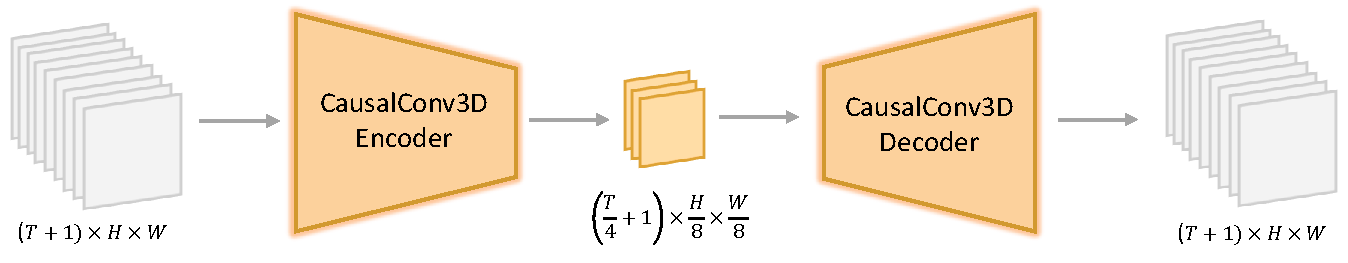
\includegraphics[width=0.95\linewidth]{figures/vae-model-arch.pdf}
    \caption{ The architecture of our 3DVAE.}
    \label{fig:vae-model-arch}
\end{figure}

\subsubsection{Training}
In contrast to most previous work \cite{polyak2024movie,chen2024od,zhou2024allegro}, we do not rely on a pre-trained image VAE for parameter initialization; instead, we train our model from scratch. 
To balance the reconstruction quality of videos and images, we mix video and image data at a ratio of $4:1$. Besides the routinely used $L_1$ reconstruction loss and KL loss $L_{kl}$, we also incorporate perceptual loss $L_{lpips}$ and GAN adversarial loss $L_{adv}$ \cite{esser2021taming} to enhance the reconstruction quality. The complete loss function is shown in Equation \ref{eq:vae-loss}.

\begin{equation}
    \label{eq:vae-loss}
    \text{Loss} = L_{1} + 0.1 L_{lpips} + 0.05 L_{adv} + 10^{-6} L_{kl}
\end{equation}

During training, we employ a curriculum learning strategy, gradually training from low-resolution short video to high-resolution long video. To improve the reconstruction of high-motion videos, we randomly choose a sampling interval from the range $1 \sim 8$ to sample frames evenly across video clips.

\subsubsection{Inference}
Encoding and decoding high-resolution long videos on a single GPU can lead to out-of-memory (OOM) errors. To address this, we use a spatial-temporal tiling strategy, splitting the input video into overlapping tiles along the spatial and temporal dimensions. Each tile is encoded/decoded separately, and the outputs are stitched together. For the overlapping regions, we utilize a linear combination for blending. This tiling strategy allows us to encode/decode videos in arbitrary resolutions and durations on a single GPU.

We observed that directly using the tiling strategy during inference can result in visible artifacts due to inconsistencies between training and inference. To solve this, we introduce an additional finetuning phase where the tiling strategy is randomly enabled/disabled during training. This ensures the model is compatible with both tiling and non-tiling strategies, maintaining consistency between training and inference. 

\begin{figure}[ht]
    \centering
    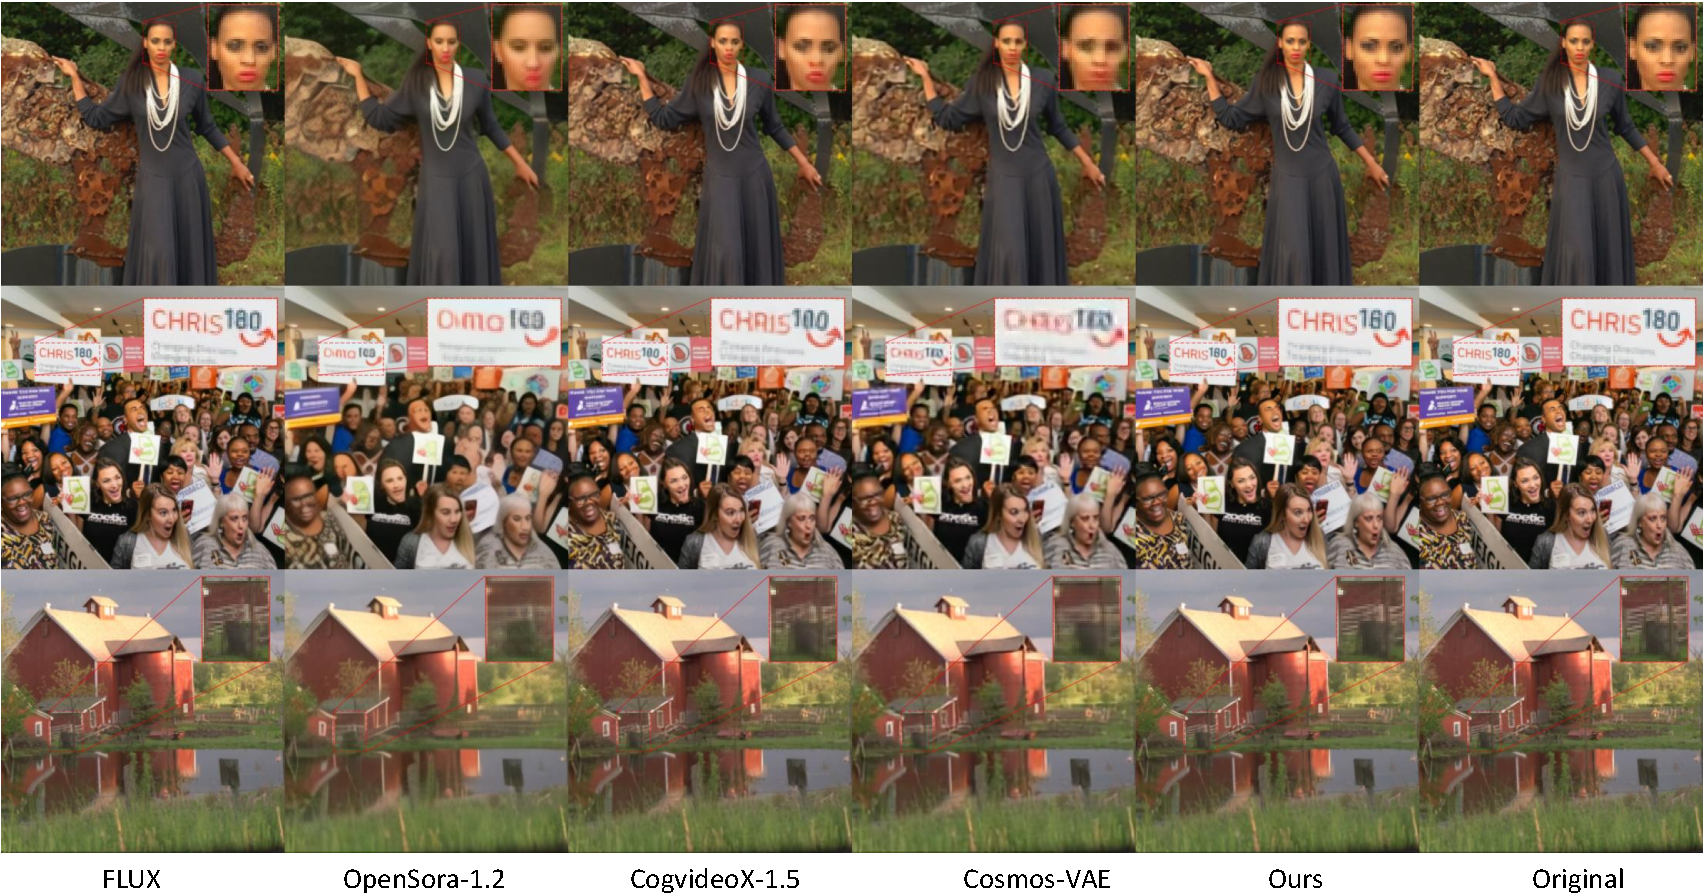
\includegraphics[width=\linewidth]{figures/vae-sota-cmp.pdf}
    \caption{VAE reconstruction case comparison.}
    \label{fig:vae-sota-cmp}
\end{figure}

Table \ref{tab:sota_vae} compares our VAE with open-source state-of-the-art VAEs. On video data, our VAE demonstrates a significantly higher PSNR compared to other video VAEs. On images, our performance surpasses both video VAEs and image VAE. Figure \ref{fig:vae-sota-cmp} shows several cases at $256 \times 256$ resolution. Our VAE demonstrates significant advantages in text, small faces, and complex textures.
%Table \ref{tab:sota_vae} compares our VAE with open-source state-of-the-art VAEs. On video data, our VAE demonstrates a significantly higher PSNR compared to other video VAEs, achieving performance comparable to frame-wise image VAE while maintaining a 4x higher temporal compression. On images, our PSNR not only surpasses that of other video VAEs but also exceeds that of image VAE. Figure \ref{fig:vae-sota-cmp} shows several cases at $256 \times 256$ resolution. It is evident that our VAE demonstrates significant advantages in  text, small faces, and complex textures.


\begin{table*}[ht]
\renewcommand{\arraystretch}{1.2}
\small
\centering  
\caption{VAE reconstruction metrics comparison.}
\begin{tabular}{lcccc}
\toprule
\multirow{2}{*}{Model} & Downsample  & \multirow{2}{*}{$|z|$} & ImageNet (256$\times$256)
& MCL-JCV (33$\times$360$\times$640) \\
& Factor & & PSNR$\uparrow$ & PSNR$\uparrow$ \\
\midrule
%FLUX-VAE~\cite{FLUX}                   & $1 \times 8 \times 8$ & 16 & 32.70 & 37.87 \\
FLUX-VAE~\cite{FLUX}                   & $1 \times 8 \times 8$ & 16 & 32.70 & - \\
\midrule
OpenSora-1.2~\cite{opensora}           & $4 \times 8 \times 8$ & 4  & 28.11 & 30.15 \\
CogvideoX-1.5~\cite{yang2024cogvideox} & $4 \times 8 \times 8$ & 16 & 31.73 & 33.22 \\
Cosmos-VAE~\cite{cosmos}               & $4 \times 8 \times 8$ & 16 & 30.07 & 32.76 \\
Ours                                   & $4 \times 8 \times 8$ & 16 & 33.14 & 35.39 \\
\bottomrule
\end{tabular}
\label{tab:sota_vae}
\end{table*}
